\documentclass[conference]{IEEEtran}
\IEEEoverridecommandlockouts
% The preceding line is only needed to identify funding in the first footnote. If that is unneeded, please comment it out.
\usepackage{cite}
\usepackage{amsmath,amssymb,amsfonts}
\usepackage{algorithmic}
\usepackage{graphicx}
\usepackage{textcomp}
\usepackage{xcolor}
\usepackage[export]{adjustbox}

\newcommand{\mycomment}[1]{}

\def\BibTeX{{\rm B\kern-.05em{\sc i\kern-.025em b}\kern-.08em
    T\kern-.1667em\lower.7ex\hbox{E}\kern-.125emX}}


\begin{document}


\title{EE0009445 Modeling the Integration of Marine Energy into Microgrids\\

\vspace{10pt}
\footnotesize{Deliverable 5.2.1 - March \\ Open-source PSS®E dynamic model of selected MHK device(s) with model agreement within 80\% target for similarity performance metrics.}}

\maketitle
% \centering
%\footnote{Alexander Barajas-Ritchie, Shuvankar Podder, Eduardo Cotilla-Sanchez, Yue Cao, Saptarshi Bhattacharya}


% \section{Deliverable 5.2.1}

% \textbf{Open-source PSS®E dynamic model of selected MHK device(s) with model agreement within 80\% target for similarity performance metrics.}



\section*{Introduction}

    Marine energy technologies—particularly Wave Energy Converters (WECs)—hold promise for decarbonizing remote coastal and islanded communities. However, their grid integration presents technical challenges, especially in microgrids with limited inertia and voltage support. This deliverable contributes to the broader EE0009445 project by advancing dynamic modeling strategies for WEC-grid interaction and testing their behavior across multiple software environments.
    
    While initial modeling efforts in Deliverable 5.1.1 utilized PowerDynamics.jl for dynamic simulations, the project has since pivoted to PowerFactory due to its relevance in Alaskan grid contexts and its industry adoption for utility-scale modeling. PowerFactory models now serve as the primary grid simulation platform for the project.
    
    In this work, we developed a dynamic Simulink model of a WEC system, including inverter control and wave-to-grid behavior. To enable cross-platform integration, this model was exported as a Functional Mock-up Unit (FMU). In PowerFactory, a custom Composite Model framework was used to import and simulate the FMU, allowing side-by-side comparison of Simulink and PowerFactory behavior under identical grid fault conditions.
    
    The central objective of this deliverable is to evaluate “model agreement”—defined as similarity in dynamic response (e.g., active power, voltage, current) between Simulink and PowerFactory models under identical disturbances. A three-phase short-circuit fault was introduced in both environments to test the WEC system’s transient behavior and recovery characteristics.
    
    Finally, all models, simulation data, and comparison scripts have been released under an open-source license and are available via the project GitHub repository.
    


\section*{WEC Dynamic Model (Simulink)}

    We used WEC-Sim to emulate the behavior of a wave energy converter. The Pierson-Moskowitz wave spectrum model was used to generate an irregular wave model with an average period of 8s and an average wave height of 8m. A permanent magnet linear generator was modeled as the power-take-off unit.  A back-to-back power electronic converter was modeled as the power conditioning unit between the wave energy converter and the grid. A supercapacitor energy storage model was used to smooth out the output power variation of the linear generator. The report of deliverable 5.3.1 describes the detailed modeling of the power electronics interfaced wave energy converter. 
    A standalone functional mock-up unit (FMU) was exported from the Simulink model to establish a connection between Simulink and PowerFactory. A Functional Mockup Unit (FMU) is a standardized self-contained file that encapsulates a simulation model. It is based on the Functional Mock-up Interface (FMI) standard, which enables the exchange and co-simulation of dynamic models across different tools. 

    
\section*{PowerFactory}
    
    For this deliverable, we used PowerFactory, a grid modeling software developed by DIgSILENT. Widely adopted in both industry and academia, PowerFactory supports load flow, RMS, and EMT simulations, making it a reliable platform for validating dynamic behavior. As an industry-standard tool, it enables robust model development and the production of credible results.
    
    To provide a consistent grid environment for simulation, we utilized the standard IEEE 14-bus system—a pre-configured test network included in PowerFactory. This system is well-understood, stable, and frequently used in validation studies, making it an ideal baseline for integration testing.
    
    \begin{figure}[t]
        \centering
        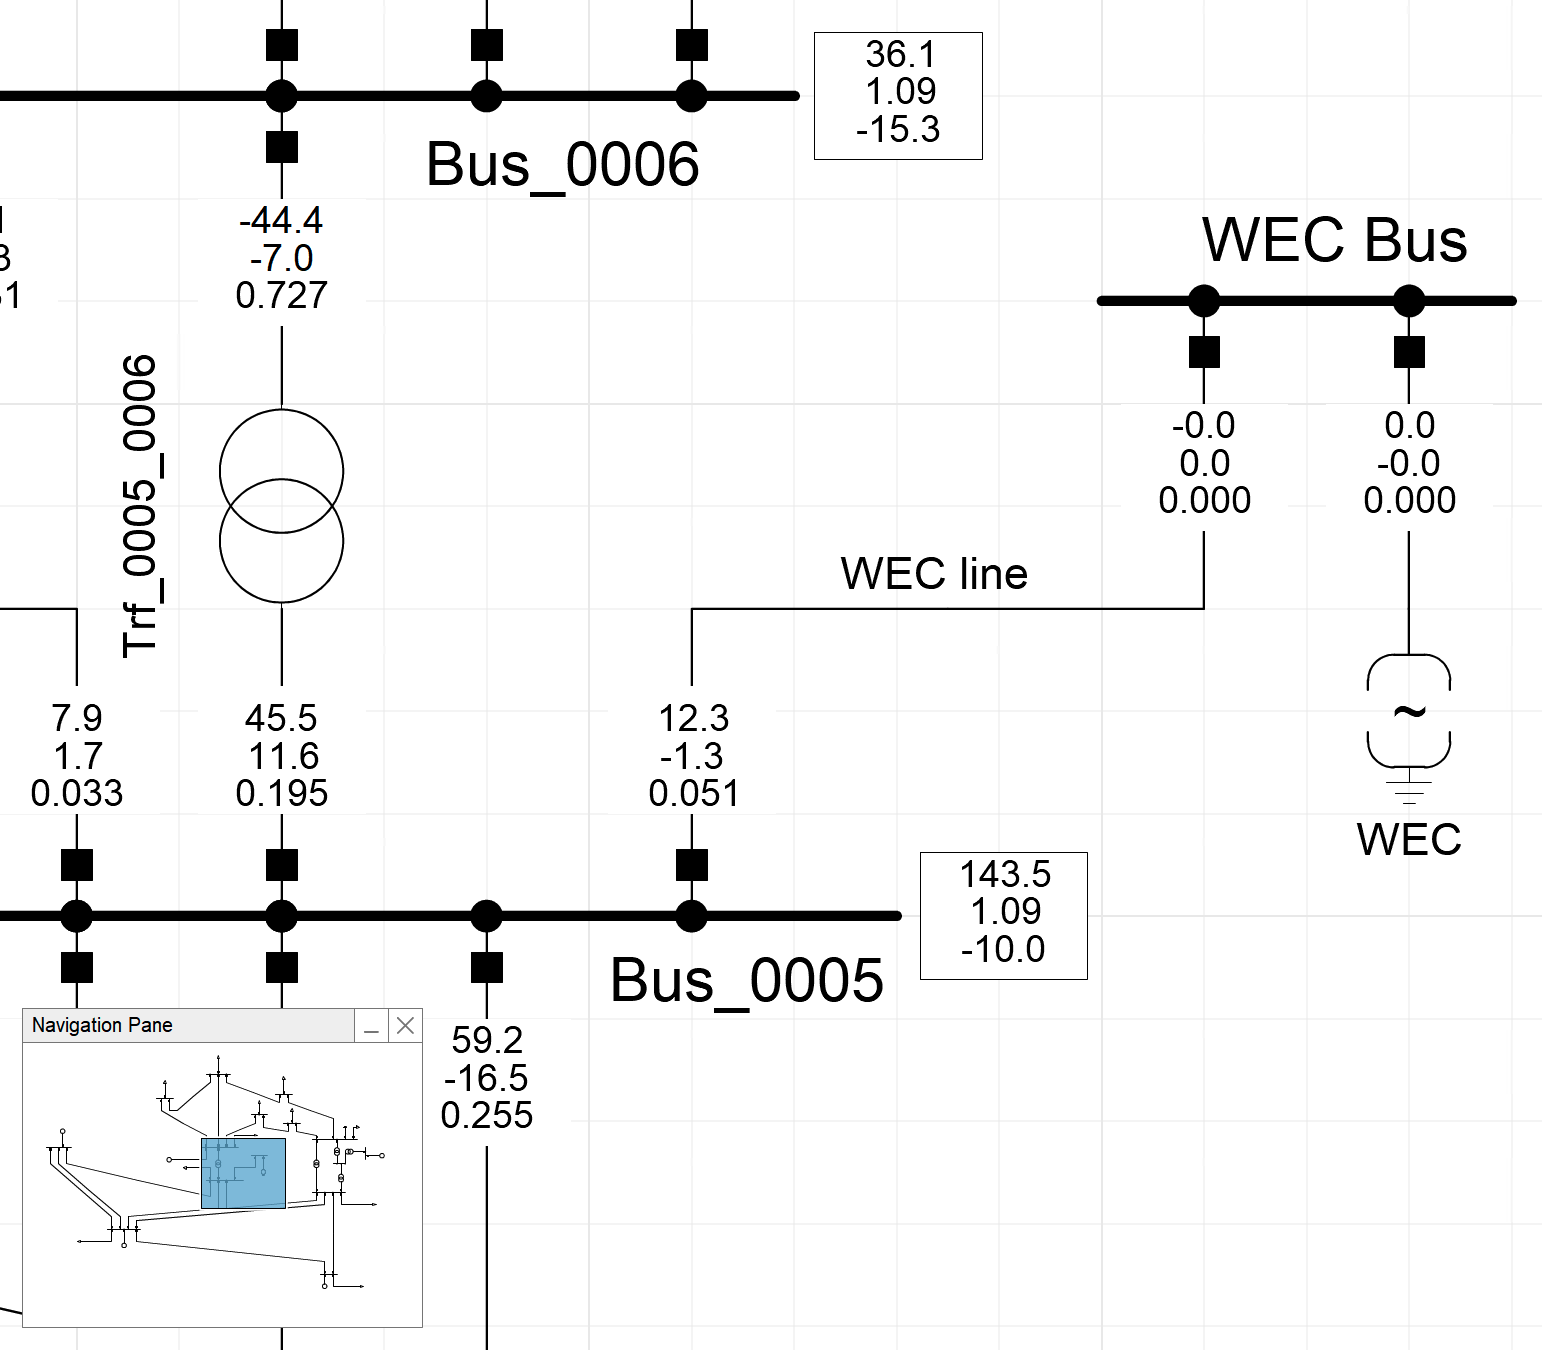
\includegraphics[width=0.8\linewidth,frame]{Figs/5_2_1/WEC_Bus_SLD.png}
        \caption{Modified IEEE 14-bus System with WEC Integration}
        \label{fig:WEC_bus_SLD}
    \end{figure}
    
    To interface our Simulink-based WEC model with the PowerFactory environment, we used a User-Defined Composite Model. Composite Models in PowerFactory are flexible templates built from slots and signals, allowing external models—such as FMUs—to interact with the grid in real-time simulation.
    
    Our WEC-FMU-Composite-Frame, shown in Figure~\ref{fig:comp_model}, includes a \texttt{Vabc} slot to read the three-phase voltage at the point of connection. This voltage is passed as an input signal \texttt{u} to the FMU block, which contains the pre-compiled Simulink model. The FMU outputs a corresponding three-phase current signal, injected into the grid via an AC Current Source block, co-located with the original voltage measurement point.
    
    \begin{figure}[t]
        \centering
        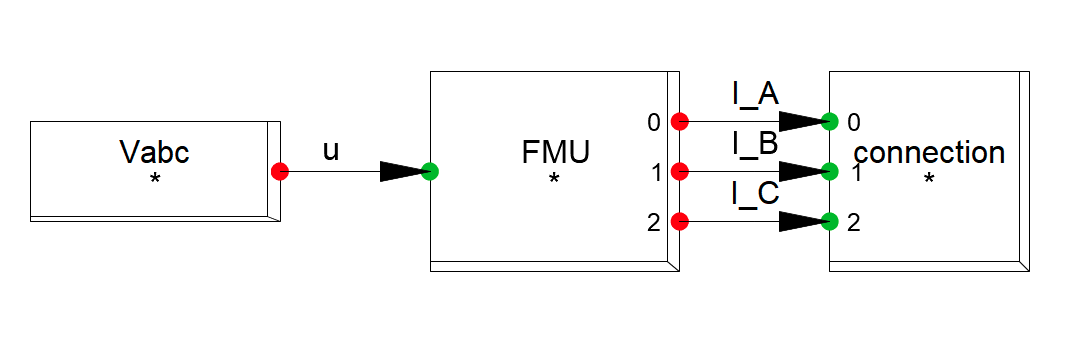
\includegraphics[width=1.0\linewidth]{Figs/5_2_1/Composite_Model.png}
        \caption{User-Defined Composite Model in PowerFactory}
        \label{fig:comp_model}
    \end{figure}
    
    This integration strategy was motivated by the need to re-use the WEC model already developed and tested in Simulink. By exporting the Simulink model as a Functional Mock-up Unit (FMU), we retained the original system dynamics while gaining compatibility with PowerFactory. This allowed us to leverage the respective strengths of both platforms—Simulink for detailed control system modeling and PowerFactory for grid-level dynamic studies—without having to reimplement models from scratch and potentially introducing some errors. It also made cross-platform comparisons more meaningful, since both environments were referencing the exact same model.
    
    The FMU-based integration assumes that the WEC model operates as a current source and maintains a fixed internal power generation profile. At present, the FMU is not synchronized to PowerFactory’s internal simulation clock, and does not update based on wave conditions in real time. Future improvements will aim to address this by synchronizing the simulation clocks and dynamically feeding wave conditions into the FMU during runtime.
    
    To facilitate integration, we modified the IEEE 14-bus case by adding an extra bus (WEC Bus), a new transmission line (WEC Line), and the AC Current Source representing the WEC system. These elements were derived from Bus 5 and Line 4–5 to maintain consistency in voltage base and simplify impedance tuning. The WEC system was connected at Bus 5, a reasonable proxy for a remote or distribution-level connection point in a real-world microgrid.
    
    
        

\section*{Model Agreement}

    \subsubsection{Fault set-up}

        To compare the behavior of our models across both software environments, we applied a similar fault scenario to observe their dynamic responses.

        Fault scenarios are a valuable tool for assessing dynamic stability and the response of control systems under grid disturbances. In our case, this test helps verify whether the model behaves consistently across platforms—specifically, whether the PowerFactory model responds similarly to our original Simulink-based implementation.
        
        In PowerFactory, we used the fault parameters listed in Table \ref{table:pf_fault}. The fault was designed to introduce a significant, yet recoverable, disturbance to the system. This allowed us to observe the coupling between the WEC and the grid under stress conditions, particularly how the WEC responds to a drop in bus voltage and how it injects current during the transient period.
        
        By applying the same type of disturbance in both environments, we aim to evaluate whether the dynamic characteristics—such as current injection, voltage dip response, and system recovery—are consistent across modeling tools.
        
        \begin{table}
            \centering
            \caption{Fault Parameters - PowerFactory}
            \begin{tabular}{|l|l|}
            \hline
            \textbf{Parameter} & \textbf{Value} \\ \hline
            Fault Type & 3-phase short circuit \\ \hline
            Fault Resistance & 0.5 $\Omega$ \\ \hline
            Fault Reactance & 0.5 $\Omega$ \\ \hline
            Fault Location & WEC Bus \\ \hline
            Fault Duration & 11.5 s – 12.0 s (within 15 s simulation) \\ \hline
            \end{tabular}
            \label{table:pf_fault}
        \end{table}

        
        
        The Simulink fault parameters are listed in Table II. A step block was used to emulate the voltage failure in the grid. We created a voltage dip of 0.2 p.u. in the grid voltage. The fault duration is 0.5s, similar to the PF simulation. A ramp block was used during the voltage recovery to make the voltage recovery a bit slow, as we observed for the 14-bus system.    \begin{table}
            \centering
            \caption{Fault Parameters - Simulink}
            \begin{tabular}{|l|l|}
            \hline
            \textbf{Parameter} & \textbf{Value} \\ \hline
            Fault Type & 3-phase short circuit \\ \hline
            Voltage dip & 0.2 p.u  \\ \hline
            Fault Location & Point of Common coupling \\ \hline
            Fault Duration & 11.5 s – 12.0 s (within 15 s simulation) \\ \hline
            \end{tabular}
            \label{table:pf_fault}
        \end{table}

\begin{figure}[t]
            \centering
            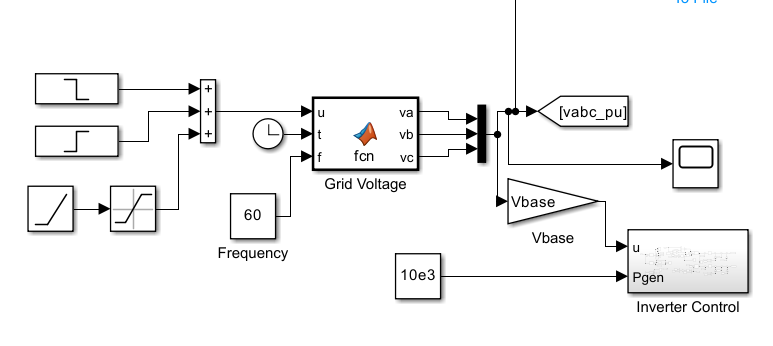
\includegraphics[width=1.0\linewidth, frame]{grid voltage emulation.png}
            \caption{Grid fault creation in Simulink}
            \label{fig:P}
        \end{figure}


        \mycomment{might need to explain some parameters differences, or not? }

    \vspace{10pt}
    
    \subsubsection{Comparison and Model Agreement Analysis}
    
    To evaluate model agreement, we compare the time-series responses from PowerFactory and Simulink simulations under identical three-phase fault conditions at the WEC connection point. Four primary metrics were assessed:
    
    \begin{itemize}
        \item \textbf{Active Power (P)} — measured at the output of the WEC system
        \item \textbf{Reactive Power (Q)} — measured at the output of the WEC system
        \item \textbf{Three-phase Voltage (Vabc)} — measured at the WEC bus
        \item \textbf{Three-phase Current (Iabc)} — measured at the point of current injection
    \end{itemize}
    
    These signals allow us to characterize both the disturbance observed by the WEC and its dynamic response. We analyze each in terms of (1) response magnitude during the fault, and (2) recovery time—defined here as the time taken to return to 90\% of the pre-fault value.
    
    \paragraph{Active Power} Both models show similar behavior during and after the fault. The minimum power output during the fault was -0.03 pu in both cases, and the power returned to 90\% of nominal in 1.002 seconds (Simulink) and 1.004 seconds (PowerFactory), demonstrating close alignment in dynamic control response.
    
    \begin{figure}[t]
        \centering
        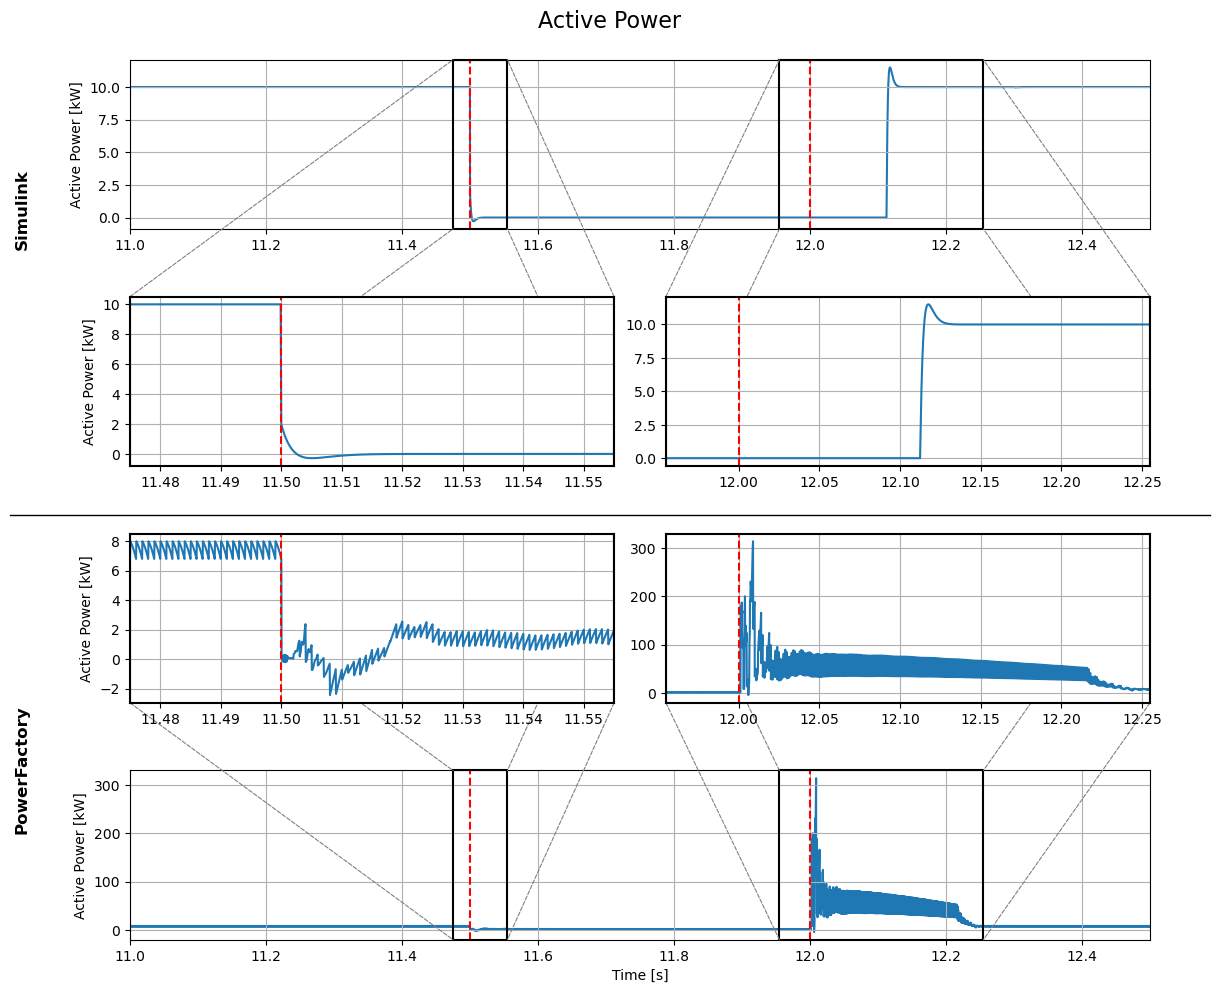
\includegraphics[width=1.0\linewidth, frame]{Figs/5_2_1/p.png}
        \caption{Active power behavior comparison}
        \label{fig:P}
    \end{figure}
    
    \paragraph{Three-phase Voltage (Vabc)} The simulated grid voltage at the WEC bus shows a similar dip and recovery profile in both platforms. While there are some differences in the depth of the voltage sag—likely due to platform-specific fault modeling and numerical solvers—the recovery times are within 10 ms of each other.
    
    \begin{figure}[t]
        \centering
        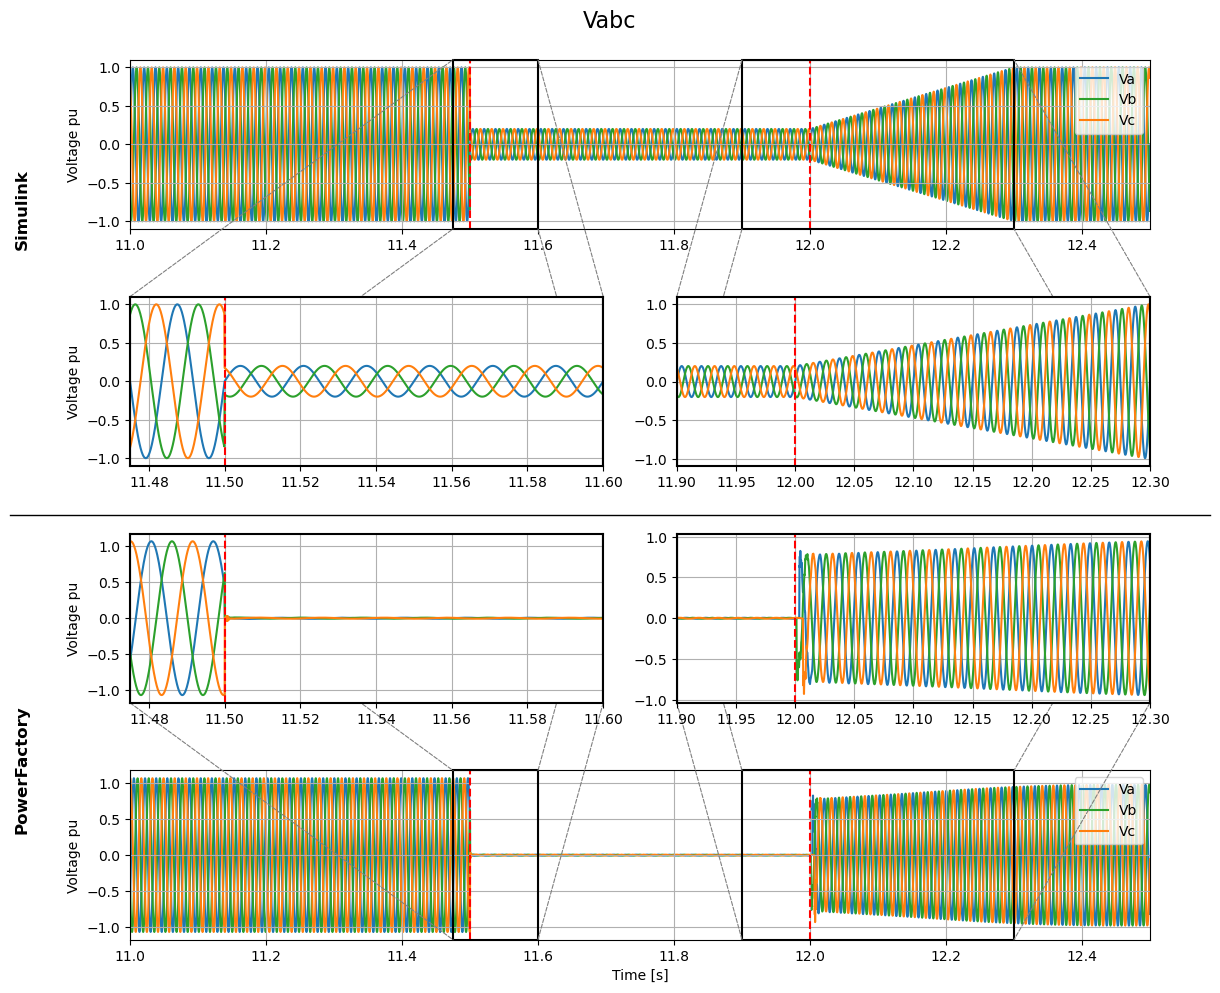
\includegraphics[width=1.0\linewidth, frame]{Figs/5_2_1/Vabc.png}
        \caption{Three-phase voltage response comparison}
        \label{fig:V}
    \end{figure}
    
    \paragraph{Three-phase Current (Iabc)} The current response also demonstrates similar dynamic behavior, though PowerFactory reports a slightly larger peak during the fault event. The recovery trajectory is consistent across all phases, with <20 ms difference in recovery times.
    
    \begin{figure}[t]
        \centering
        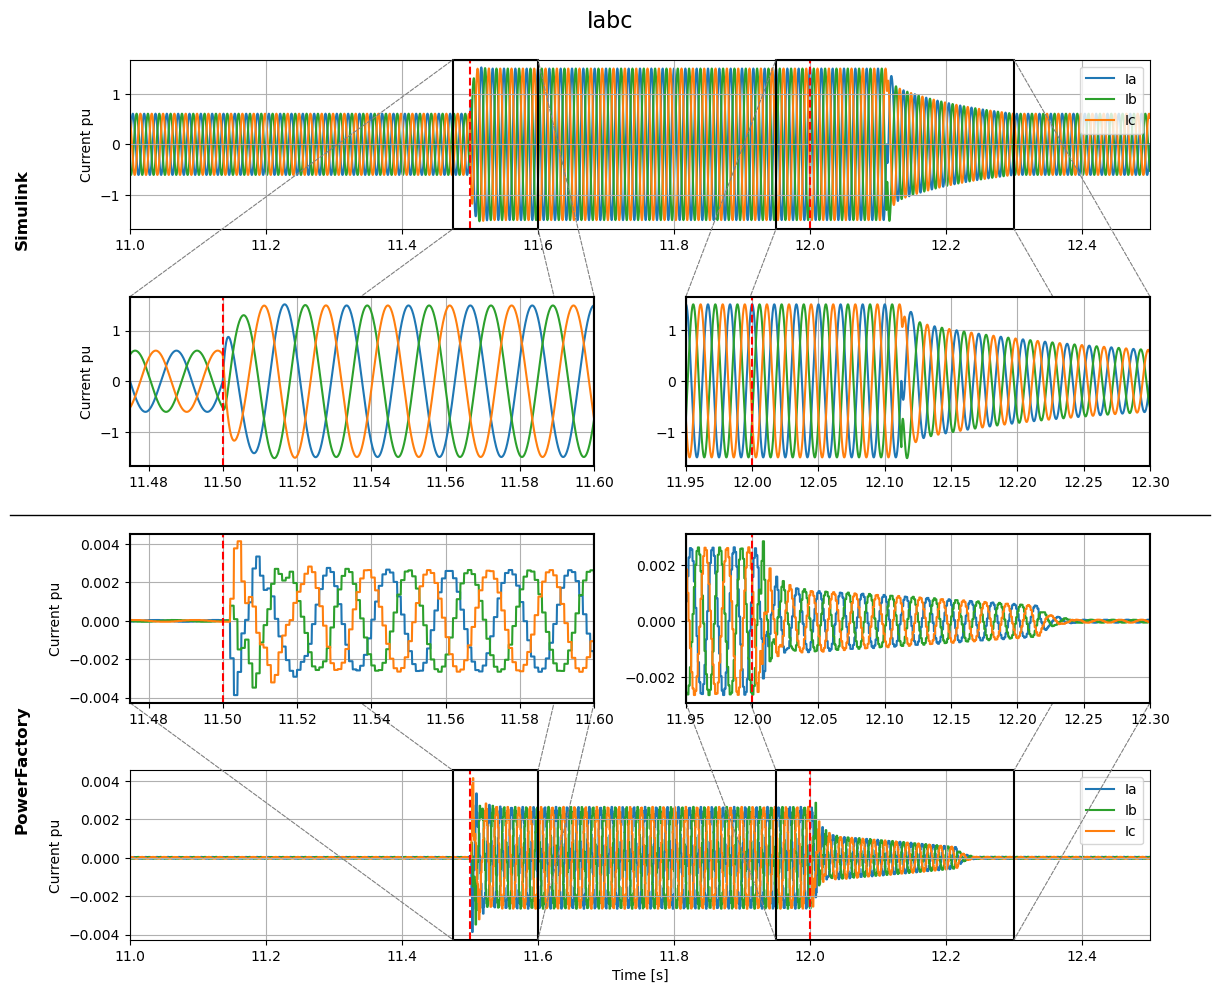
\includegraphics[width=1.0\linewidth, frame]{Figs/5_2_1/Iabc.png}
        \caption{Three-phase current response comparison}
        \label{fig:I}
    \end{figure}
    
    \paragraph{Quantitative Agreement} Across all measured quantities, we find that PowerFactory and Simulink simulations match within tight tolerances:
    \begin{itemize}
        \item \textbf{Active power recovery time difference:} 2 ms
        \item \textbf{Voltage recovery time differences:} 3–5 ms across phases
        \item \textbf{Current recovery time differences:} 1–2 ms
    \end{itemize}
    
    These results suggest that the FMU-based integration into PowerFactory preserves the essential dynamic behavior of the original Simulink WEC model. While some absolute values differ slightly—especially during fault initiation—the timing, control response, and recovery dynamics exhibit strong agreement, supporting the use of cross-platform validation.


    \begin{table}[t]
        \centering
        \caption{Summary of Key Fault Response Metrics}
        \begin{tabular}{|c|c|c|c|}
        \hline
        \textbf{Metric} & \textbf{Simulink} & \textbf{PowerFactory} & \textbf{Difference} \\
        \hline
        \textbf{P Drop (pu)} & -0.03 & -0.03 & 0.00 \\
        \textbf{P Recovery (s)} & 1.002 & 1.004 & 0.002 \\
        \hline
        \textbf{Vabc Recovery (s)} & Avg: 1.001 & Avg: 1.007 & $\sim$6 ms \\
        \textbf{Iabc Peak (pu)} & -3.93 & -6.60 & $\sim$2.7 \\
        \textbf{Iabc Recovery (s)} & Avg: 1.004 & Avg: 1.014 & $\sim$10 ms \\
        \hline
        \end{tabular}
        \label{table:agreement_metrics}
    \end{table}

\section{Discussion and Conclusion}
    
    Overall, the comparison between PowerFactory and Simulink implementations of the WEC system shows strong agreement in both qualitative behavior and quantitative metrics.
    
    Despite differences in numerical solvers and waveform resolution, the key performance indicators—such as active power drop and recovery, voltage sag response, and current injection—demonstrate alignment within milliseconds and per-unit-level tolerances.
    
    Most importantly, the cross-platform WEC model exhibited similar transient behavior during the 3-phase short circuit and consistent timing in its return to steady-state operation. This confirms that the FMU export and integration strategy successfully preserved the dynamic characteristics of the original model.

    % \noindent
    % \textbf{Code Repository:} All models and analysis scripts are available at: 
    % \url{https://github.com/barajale/Model_Comparison}



% \section{Conclusion}
\end{document}
